\documentclass{thesis}
\usepackage[margin=0.5in]{geometry}
\documentclass[a4paper,10pt,draft]{thesis}
\usepackage{physics,amsmath, amsfonts, siunitx, amssymb, graphicx, slashed,subcaption}
\usepackage[utf8]{inputenc}
\usepackage[margin=1in]{geometry}
\usepackage[hidelinks]{hyperref}
\usepackage{xr-hyper}
\newcommand{\n}[1]{\nu_{#1}}
\newcommand{\na}{\nu_\alpha}
\newcommand{\nb}{\nu_\beta}
\newcommand{\ana}{\bar{\nu}_\alpha}
\newcommand{\an}[1]{\bar{\nu}_{\text{#1}}}
\newcommand{\anb}{\bar{\nu}_\beta}
\renewcommand{\a}{\alpha}
\renewcommand{\b}{\beta}
\newcommand{\ab}{\alpha\beta}


\renewcommand{\ne}{\nu_e}
\newcommand{\nm}{\nu_\mu}
\newcommand{\nt}{\nu_\tau}
\newcommand{\ns}{\nu_s}

\newcommand{\ane}{\bar{\nu}_e}
\newcommand{\anm}{\bar{\nu}_\mu}
\newcommand{\ant}{\bar{\nu}_\tau}
\newcommand{\ans}{\bar{\nu}_s}

\newcommand{\nee}{\nu_e \to \nu_e}
\newcommand{\nem}{\nu_e \to \nu_\mu}
\newcommand{\net}{\nu_e \to \nu_\tau}
\newcommand{\nes}{\nu_e \to \nu_s}

\newcommand{\nme}{\nu_\mu \to \nu_e}
\newcommand{\nmm}{\nu_\mu \to \nu_\mu}
\newcommand{\nmt}{\nu_\mu \to \nu_\tau}
\newcommand{\nms}{\nu_\mu \to \nu_s}



\newcommand{\Pee}{P_{e  e}}
\newcommand{\Pem}{P_{e  \mu}}
\newcommand{\Pet}{P_{e  \tau}}
\newcommand{\Pes}{P_{e  s}}

\newcommand{\Pme}{P_{\mu  e}}
\newcommand{\Pmm}{P_{\mu\mu}}
\newcommand{\Pmt}{P_{\mu  \tau}}
\newcommand{\Pms}{P_{\mu  s}}


\newcommand{\Pte}{P_{P_{\tau e}}}
\newcommand{\Ptm}{P_{\tau  \mu}}
\newcommand{\Ptt}{P_{\tau  \tau}}
\newcommand{\Pts}{P_{\mu  s}}

\newcommand{\Paeae}{P_{\bar{e}  \bar{e}}}
\newcommand{\Paeam}{P_{\bar{e}  \bar{\mu}}}
\newcommand{\Paeat}{P_{\bar{e}  \bar{\tau}}}
\newcommand{\Paeas}{P_{\bar{e}  \bar{s}}}

\newcommand{\Pamae}{P_{\bar{\mu}  \bar{e}}}
\newcommand{\Pamam}{P_{\bar{\mu}  \bar{\mu}}}
\newcommand{\Pamat}{P_{\bar{\mu}  \bar{\tau}}}
\newcommand{\Pamas}{P_{\bar{\mu}  \bar{s}}}


\newcommand{\Patae}{P_{\bar{\tau}  \bar{e}}}
\newcommand{\Patam}{P_{\bar{\tau}  \bar{\mu}}}
\newcommand{\Patat}{P_{\bar{\tau}  \bar{\tau}}}
\newcommand{\Patas}{P_{\bar{\mu}  \bar{s}}}

\renewcommand{\th}[1][]{%
  \theta\ifx\\#1\\\else_\text{#1}\fi
}
\newcommand{\thm}[1][]{%
  \theta^\text{M}\ifx\\#1\\\else_\text{#1}\fi
}
\renewcommand{\t}[1]{\text{{#1}}}
\newcommand{\avg}[1]{\left\langle {#1} \right \rangle}
\newcommand*{\dm}[1][]{%
  \Delta m^2\ifx\\#1\\\else_\text{#1}\fi
}
\newcommand{\zreco}{\cos{(\theta_z^{reco})}}
\newcommand{\ztrue}{\cos{(\theta_z^{true})}}
\newcommand{\z}{\cos{(\theta_z)}}
\newcommand{\Ereco}{E^{reco}}
\newcommand{\Etrue}{E^{true}}
\newcommand{\Aeff}{A^\text{eff}}
\newcommand{\emm}{\epsilon_{\mu\mu}}
\newcommand{\emt}{\epsilon_{\mu\tau}}
\newcommand{\eet}{\epsilon_{e\tau}}
\newcommand{\eem}{\epsilon_{e\mu}}
\newcommand{\ett}{\epsilon_{\tau\tau}}
\newcommand{\ep}{\epsilon^\prime}


\begin{document}
\section{Monte Carlo normalization}
Independent researchers outside of the IceCube collaboration will not be able to more persicely
simulate the detector. The IceCube Monte Carlo is a complex and proprietary machinery, so our goal in this 
section is to come as close as we can to their Monte Carlo simulations. After we are confident that 
our code displays the same overall features as the ´offical', we normalize our results $N_{ij}^\text{sim}$ as 
\begin{align}\label{eq:MC_norm}
    N_{ij}^\text{corr} = \frac{N_{ij}^\text{null}}{N_{ij}^\text{MC}}\,.
\end{align}
For each bin $i,j$, we then obtain a correction factor which contains information that we are unable
to obtain or sufficiently incorporate. One example of such information is the systematic errors of the DOMs.
Recent IceCube data releases do not include such information. Since the systematic errors are affecting the 
event count on a bin-by-bin basis, they can in theory drastically modify the binned results. Another example of
an error source what will be remedied by this method is the flux. We are using a fairly simple model of the atmospheric 
flux that excludes prompt flux. The IceCube collaboration use several different flux models which are initialized 
by a parametrization of the cosmic ray flux.\footnote{Included in the cosmic ray models are e.g. the pion to kaon 
ratio, which are often used as a nuisance parameter. By not being able to include this in our error analysis, our method will 
be limited to only consider the overall flux normalization, rather than the components that produce the flux in the first place.}
%TODO: maybe rambling?

In Fig.~\ref{fig:IC_MC_norm}, we present the Icecube Monte Carlo obtained from their 2020 sterile analysis~\cite{IC2020}, along
with our null hypothesis times a constant factor.  We deemed these shapes to be satisfactory, thus allowing us to multiply Eq.~\ref{eq:ICevents} by the 
correction factors of Eq.~\ref{eq:MC_norm}. We now arrive to our final event count
\begin{align}\label{eq:Nth}
    N_{ij} &= \frac{N_{ij}^\text{null}}{N_{ij}^\text{MC}} T \int_{(\cos{\theta_z^r})_i}^{(\cos{\theta_z^r})_{i+1}} \dd \cos{\theta^r_z} \int_{E^r_{j}}^{E^r_{j+1}} \dd E^r \int_0^\pi R(\theta^r,\theta^t) \dd \cos{\theta^t} \int_0^\infty R(E^r,E^t) \dd E^t
    \times \left[ \sum_\beta \phi_\beta^\text{det}  A^\text{eff}_\beta\right]\,,
\end{align}
\begin{figure}
    \centering
    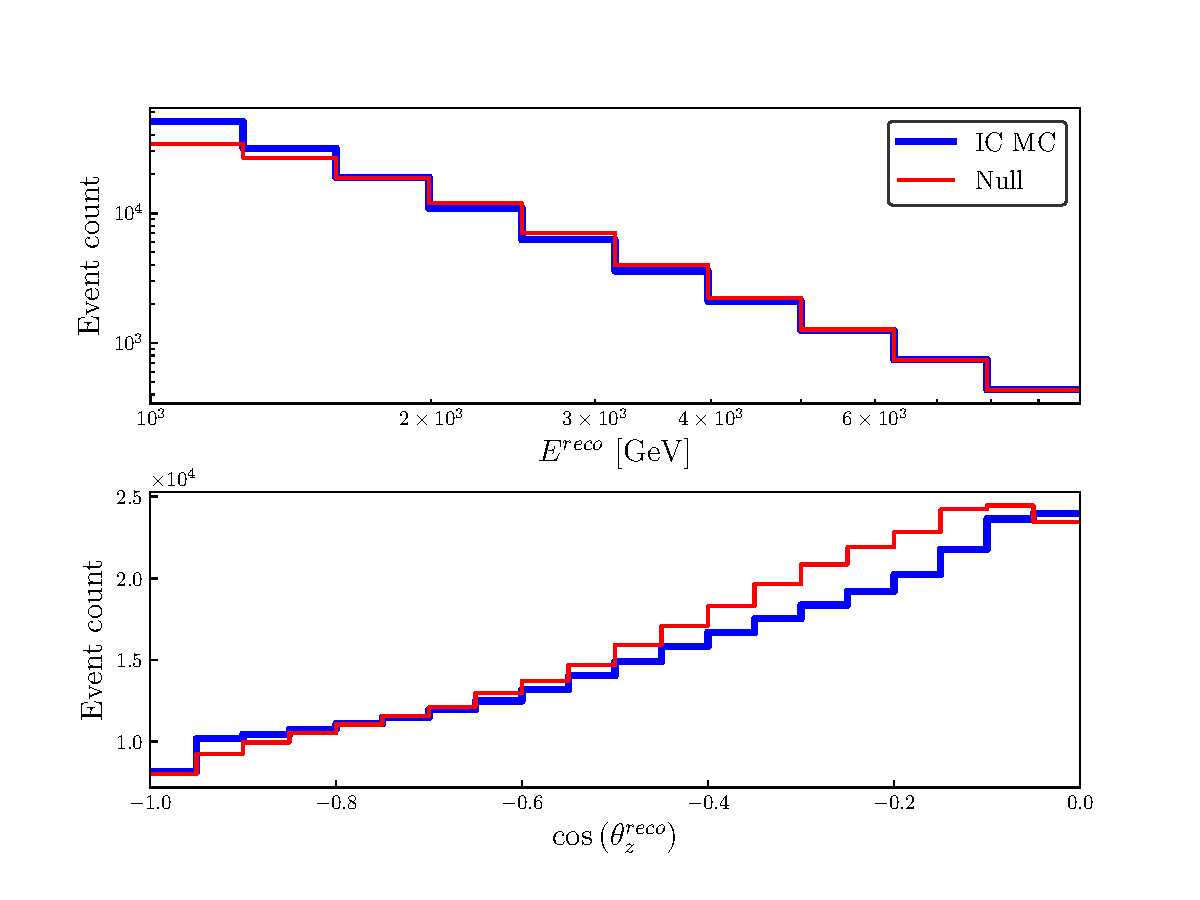
\includegraphics[width=0.8\linewidth]{figures/IC_MC_norm.pdf}
    \caption{IceCube Monte Carlo, binned in $\Ereco$ and $\zreco$. We compare this with our simulations shown as ´Null' in the plots.}\label{fig:IC_MC_norm}
\end{figure} 

\section{Sterile hypothesis}
With the null normalized, we are now in good shape to study the sterile effect on the probabilities, and how that compares to data.
First, let us see how the collected data from Fig.~\ref{fig:IC_data} deviates from the predicted $3\nu$ oscillations.
\begin{figure}
    \centering
    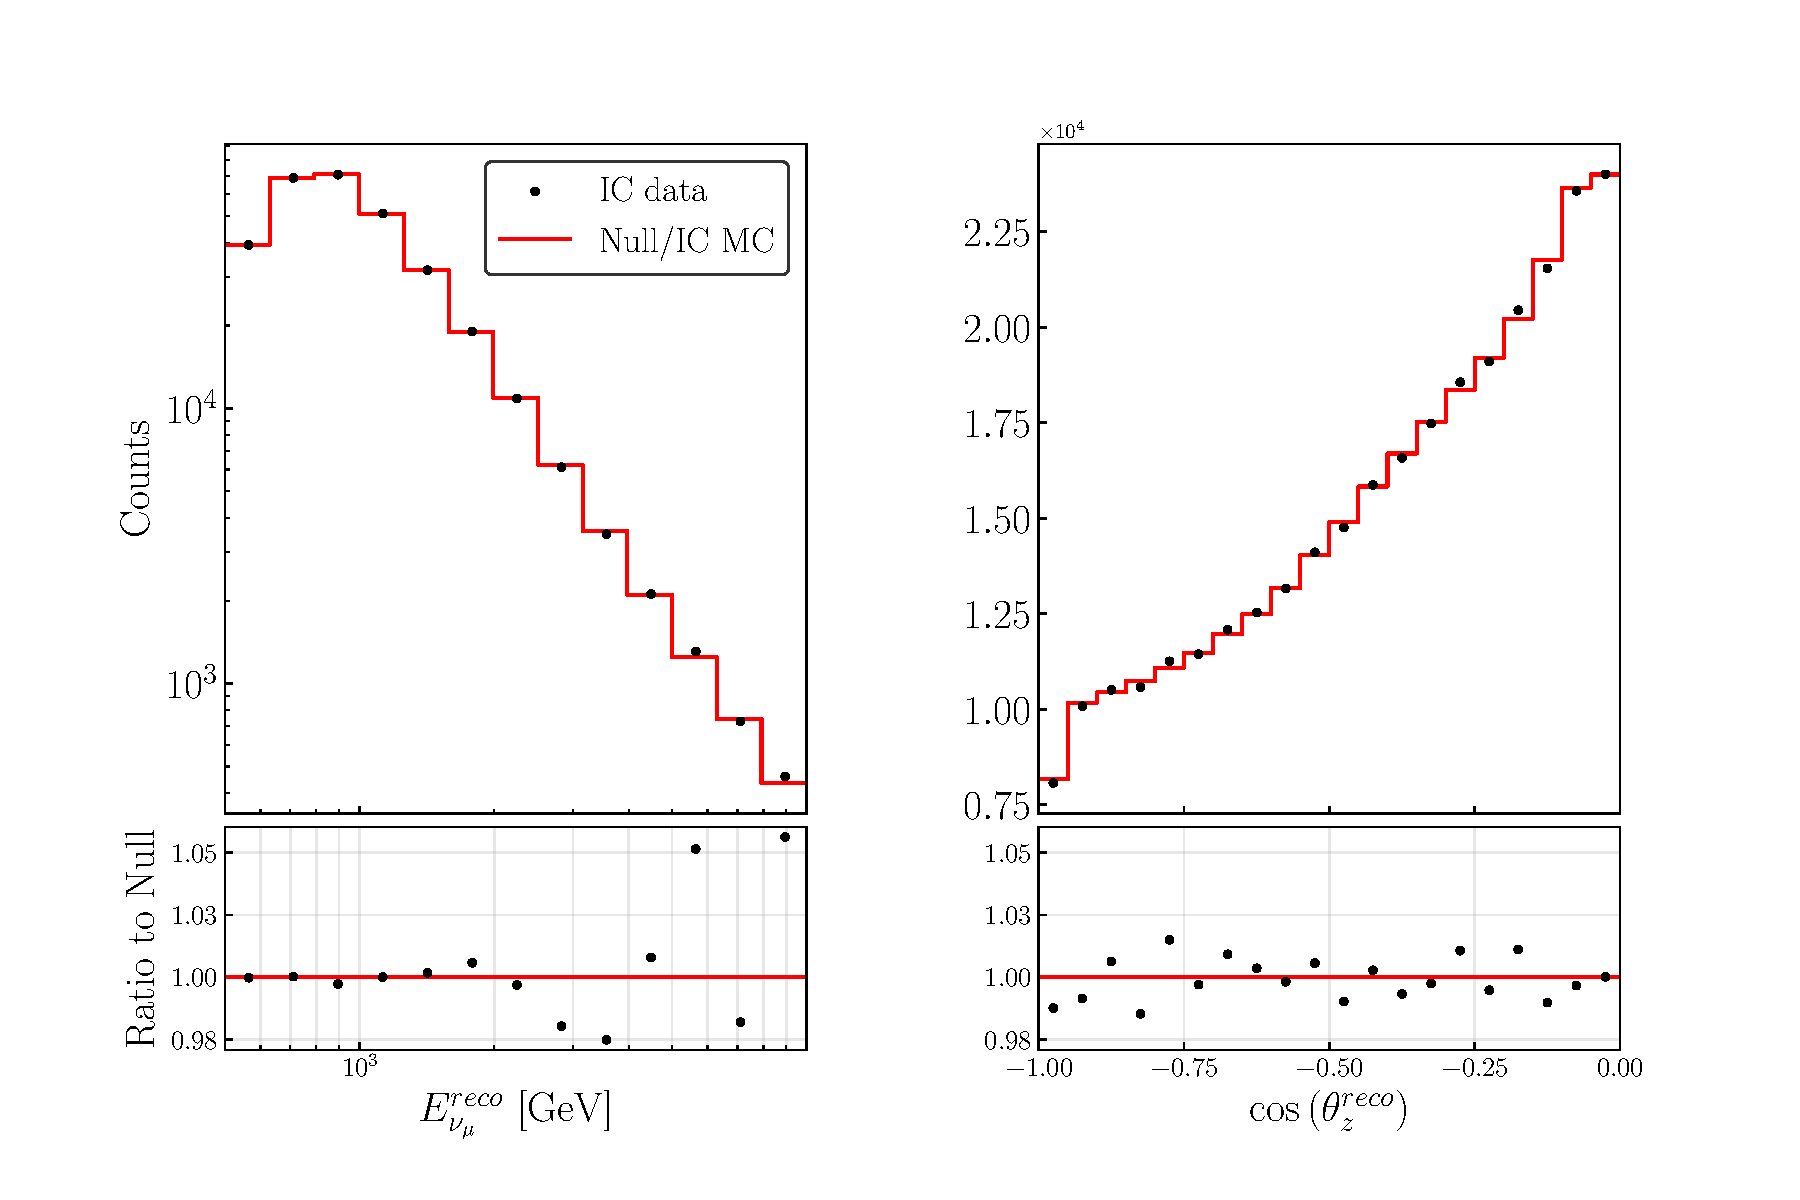
\includegraphics[width=0.8\textwidth]{figures/IC_rates.pdf}
    \caption{}\label{fig:IC_rates}
\end{figure}
Fig.~\ref{fig:IC_rates} shows an impressive agreement to the standard $3\nu$ oscillation picture, with the largest deviations of $~6\%$
for neutrinos close to double-digit \si{\TeV} values. In zenith, the data only deviates $\pm 1\%$. Recalling the \si{\TeV} disappearance from 
Fig.~\ref{fig:sterile_resonance}, we see that we have a similar deficiency found in the data at $4 \si{TeV}$. Thus, we expect the best fitting 
sterile hypothesis to include a $\dm[41]$ that places the resonant disappearance in the same region. From Fig.~\ref{fig:resonance_shift}, we see
that a mass of $\dm[41] = \SI{1.5}{\eV \squared}$ achieves this. 

\section{$\chi^2$}
For our analyses, we define our $\chi^2$ as
\begin{align} \label{eq:chisq}
    \chi^{2}(\hat{\theta},\alpha,\beta)=\sum_{ij} \frac{\left(N^\text{th}-N^\text{data}\right)_{ij}^{2}}
    {\left(\sigma^\text{data}_{ij}\right)^{2} + \left(\sigma^\text{syst}_{ij}\right)^{2}}+ 
    \frac{(1-\alpha)^2}{\sigma_\alpha^2} + \frac{\beta^2}{\sigma_\beta^2}\,
\end{align}
where we minimize over the model parameters $\hat{\theta} \in \{\dm[41], \theta_{24}\}$, the penalty terms $\alpha$ and $\beta$.
$N_{ij}^\text{th}$ is the expected number of events from theory, and $N_{ij}^\text{data}$ is the observed number of events in that bin. 
We set $\sigma_\alpha = 0.25$ as the atmospheric flux normalization error, and $\sigma_\beta = 0.04$ as the zenith angle slope error~\cite{hondapaper}. 
The observed event number has an associated Poissonian uncertainty $\sigma_{ij}^\text{data} = \sqrt{N_{ij}^\text{data}}$.
For IceCube, the event count takes the form
\begin{align}
    N^\text{th}_{ij} = \alpha\left[1+\beta (0.5 + \zreco_i )\right] N_{ij}(\hat{\theta})\,,
\end{align}
with $N_{ij}(\hat{\theta})$ from Eq.~\ref{eq:Nth}. Here, the term $ \beta (0.5 + \zreco_i )$ allows the event distribution to rotate around the median zenith angle of $\zreco = -0.5$.

\end{document}